\documentclass[english,11pt]{article}
\usepackage[T1]{fontenc}
\usepackage[latin9]{inputenc}
\usepackage{geometry}
\usepackage{graphicx}
\usepackage{subcaption} % to plot subfigure
\usepackage[linesnumbered,ruled,vlined]{algorithm2e}
\geometry{verbose,tmargin=2.5cm,bmargin=2.5cm,lmargin=2.5cm,rmargin=2.5cm}
\usepackage{amsmath}
\usepackage{babel}
\begin{document}



\title{COMP 540 HW 01 }

\author{Lyu Pan (lp28), Yuhui Tong (yt30)}
\maketitle



%%%%%%%%%%%%%%%%%%%%%%%%%%%%%%%%%%%%
%%%%%%%%%% part 0 %%%%%%%%%%%%%%%%%%
%%%%%%%%%%%%%%%%%%%%%%%%%%%%%%%%%%%%

\part*{0. Background Refresher}

\subsection*{0.0 Samplers} 

\begin{figure}[h]
\centering
\begin{subfigure}{.5\textwidth}
\centering
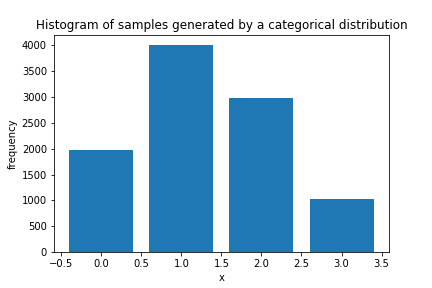
\includegraphics[width=.8\linewidth]{samplefigs/fig1.png}
\end{subfigure}%
\begin{subfigure}{.5\textwidth}
\centering
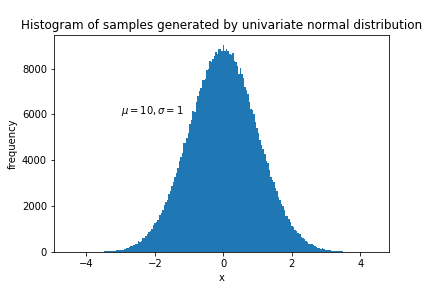
\includegraphics[width=0.8\textwidth]{samplefigs/fig2.png}
\end{subfigure}

\begin{subfigure}{.5\textwidth}
\centering
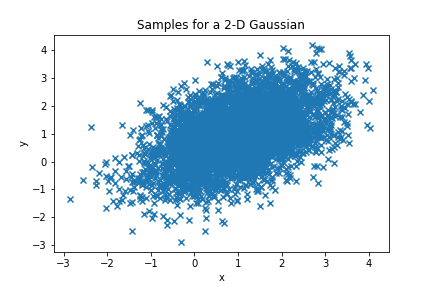
\includegraphics[width=.8\linewidth]{samplefigs/fig3.png}
\end{subfigure}%
\begin{subfigure}{.5\textwidth}
\centering

\includegraphics[width=0.8\textwidth]{samplefigs/fig4.png}
\end{subfigure}
\end{figure}


\subsection{Prove two independent Poisson random variables are also Poisson variable.}

Proof:

Given two independent random variables $X_{1}\sim P(\lambda_{1})$
and $X\sim P(\lambda_{2})$. i.e.,

\begin{equation}
P(X_{1}=m)=e^{-\lambda_{1}}\frac{\lambda_{1}^{m}}{m!},\ m=1,2,...    
\end{equation}


and

\begin{equation}
P(X_{2}=n)=e^{-\lambda_{2}}\frac{\lambda_{2}^{n}}{n!},\ n=0,1,2,...    
\end{equation}


Denote sum of them are 
\begin{equation}
X=X_{1}+X_{2}
\end{equation}

then the probability distribution of $X$ is:

\begin{eqnarray}
P(X=k) & = & \sum_{m+n=k}P(X_{1}=m,X_{2}=n) \notag \\
 & \overset{X_{1},X_{2}indep.R.V.}{=} & \sum_{m+n=k}P(X_{1}=m)P(X_{2}=n) \notag \\
 & = & \sum_{m+n=k}e^{-\lambda_{1}}\frac{\lambda_{1}^{m}}{m!}e^{-\lambda_{2}}\frac{\lambda_{2}^{n}}{n!} \notag \\
 & = & \frac{1}{k!}e^{-(\lambda_{1}+\lambda_{2})}\sum_{m+n=k}\frac{k!}{m!n!}\lambda_{1}^{m}\lambda_{2}^{n} \notag \\
 & = & \frac{1}{k!}e^{-(\lambda_{1}+\lambda_{2})}(\lambda_{1}+\lambda_{2})^{k}
\end{eqnarray}

that is, $X=X_{1}+X_{2}\sim P(\lambda_{_{1}}+\lambda_{2})$. Q.E.D.

\subsection{Proof question 2}

\begin{eqnarray}
p(x_{1,}x_{0}) & = & p(x_{1}|x_{0})p(x_{0}) \notag \\
 & = & \alpha e^{-\frac{(x_{1}-x_{0})^{2}}{2\sigma^{2}}}\alpha_{0}e^{-\frac{(x_{0}-\mu_{0})^{2}}{2\sigma_{0}^{2}}}
\end{eqnarray}

The probability distribution of $X_{1}$ is,

\begin{eqnarray}
p(x_{1}) & = & \int_{-\infty}^{\infty}p(x_{1},x_{0})dx_{0} \notag \\
 & = & \int_{-\infty}^{\infty}\alpha e^{-\frac{(x_{1}-x_{0})^{2}}{2\sigma^{2}}}\alpha_{0}e^{-\frac{(x_{0}-\mu_{0})^{2}}{2\sigma_{0}^{2}}}dx_{0} \notag \\
 & = & D\int_{-\infty}^{\infty}e^{-A[x_{0}-B]^{2}+C}dx_{0}
\end{eqnarray}
where $A,B,C,D$

\begin{eqnarray}
D & = & \alpha\alpha_{0}e^{-\frac{\mu_{0}^{2}}{2\sigma_{0}^{2}}}e^{-\frac{x_{1}^{2}}{2\sigma^{2}}}
\end{eqnarray}

\begin{equation}
A=\frac{\sigma_{0}^{2}+\sigma^{2}}{2\sigma_{0}^{2}\sigma^{2}},    
\end{equation}


\begin{equation}
B=\frac{x_{1}\sigma_{0}^{2}+\mu_{0}\sigma^{2}}{\sigma_{0}^{2}+\sigma^{2}},
\end{equation}


\begin{equation}
C=\frac{(x_{1}\sigma_{0}^{2}+\mu_{0}\sigma^{2})^{2}}{2\sigma_{0}^{2}\sigma^{2}(\sigma_{0}^{2}+\sigma^{2})}.    
\end{equation}


Making the substitution $t=\sqrt{2A}(x_{0}-B)$ gives

\begin{eqnarray}
\int_{-\infty}^{\infty}e^{-A[x_{0}-B]^{2}+C}dx_{0} & = & \int_{-\infty}^{\infty}e^{-\frac{t^{2}}{2}+C}d\frac{t}{\sqrt{2A}} \notag \\
 & = & \frac{1}{\sqrt{2A}}e^{-C}\int_{-\infty}^{\infty}e^{-\frac{t^{2}}{2}}dt \notag \\
 & = & \sqrt{\frac{\pi}{A}}e^{-C}
\end{eqnarray}
where in the second step we used $\int_{-\infty}^{\infty}e^{-\frac{t^{2}}{2}}dt=\sqrt{2\pi}$. 

Substitute the above equation to the Eq.~():

\begin{eqnarray}
p(x_{1}) & = & D\sqrt{\frac{\pi}{A}}e^{-C} \notag \\
 & = & \alpha\alpha_{0}e^{-\frac{\mu_{0}^{2}}{2\sigma_{0}^{2}}}e^{-\frac{x_{1}^{2}}{2\sigma^{2}}}\sqrt{\frac{\pi}{A}}e^{-C}
\end{eqnarray}

\subsection{question 4 eigenvalues}

\[
\boldsymbol{A}=\left[\begin{array}{cc}
13 & 5\\
2 & 4
\end{array}\right]
\]

\begin{eqnarray*}
\boldsymbol{A}\boldsymbol{X} & = & \lambda\boldsymbol{X}\\
(\boldsymbol{A}-\lambda\boldsymbol{I})\boldsymbol{X} & = & 0\\
\left[\begin{array}{cc}
13-\lambda & 5\\
2 & 4-\lambda
\end{array}\right]\boldsymbol{X} & = & 0
\end{eqnarray*}

$\lambda_{1}=3$, $\boldsymbol{X}_{1}=\left(\begin{array}{c}
-1/2\\
1
\end{array}\right)$

$\lambda_{2}=14$, $\boldsymbol{X}_{2}=\left(\begin{array}{c}
5\\
1
\end{array}\right)$

\subsection{question 5, matrix multiplication}

$A=\left[\begin{array}{cc}
1 & 2\\
3 & 4
\end{array}\right]$, $B=\left[\begin{array}{cc}
5 & 6\\
7 & 8
\end{array}\right]$, we have $(A+B)^{2}\neq A^{2}+2AB+B^{2}$ 

$A=\left[\begin{array}{cc}
0 & 1\\
0 & 1
\end{array}\right]$, $B=\left[\begin{array}{cc}
1 & 1\\
0 & 0
\end{array}\right]$ , $A,B\neq0$ and we have $AB=0$

\subsection{question 6}

\begin{eqnarray}
A^{T}A & = & (I-2uu^{T})^{T}(I-2uu^{T}) \notag \\
 & = & (I-2uu^{T})(I-2uu^{T}) \notag \\
 & = & I-2uu^{T}-2uu^{T}+4u(u^{T}u)u^{T} \notag \\
 & = & I
\end{eqnarray}

\subsection{convex function}

\subsection{entropy of categorical distribution}

The entropy of a categorical distribution on $K$ values is 

\begin{eqnarray}
H(p) & = & -\sum_{i=1}^{K}p_{i}\log(p_{i}),
\end{eqnarray}
with constraint that 
\begin{equation}
\sum_{i=1}^{K}p_{i}=1.    
\end{equation}


Using Lagrange Multiplier, one can combine the above two equations
into:

\begin{equation}
L(p,\lambda)=-\sum_{i=1}^{K}p_{i}\log(p_{i})+\lambda(\sum_{i=1}^{K}p_{i}-1).    
\end{equation}


Taking derivative of all unknown variables gives:

\begin{equation}
\frac{\partial L}{\partial p_{i}}=-(\log p_{i}+1)+\lambda=0,\ i=1,2,...    
\end{equation}


Substituting $p_{i}$ with $\lambda$ yields


\begin{equation}
p_{i}=\frac{1}{K},\ i=1,2,...,K.    
\end{equation}

Q.E.D.



%%%%%%%%%%%%%%%%%%%%%%%%%%%%%%%%%%%%
%%%%%%%%%% part 1 %%%%%%%%%%%%%%%%%%
%%%%%%%%%%%%%%%%%%%%%%%%%%%%%%%%%%%%


\part*{1. Locally weighted linear regression.}

\subsection*{1.1 Expression of $J(\theta)$}

Define $\boldsymbol{X},$ $\boldsymbol{W}$ in the following way:


\begin{equation}
\boldsymbol{X}=\left[\begin{array}{c}
----\left(x^{(1)}\right)^{T}----\\
----\left(x^{(2)}\right)^{T}----\\
\vdots\\
----\left(x^{(m)}\right)^{T}----
\end{array}\right]\Longleftrightarrow\boldsymbol{X}_{i,j}=(x^{(i)})_{j}    
\end{equation}

 
\begin{equation}
\boldsymbol{W}=\left[\begin{array}{cccc}
w^{(1)}\\
 & w^{(2)}\\
 &  & \ddots\\
 &  &  & w^{(m)}
\end{array}\right]\Longleftrightarrow\boldsymbol{W}_{i,j}=\delta_{i,j}w^{(i)}    
\end{equation}


Substituting $\boldsymbol{X},$ $\boldsymbol{W}$ into $(\boldsymbol{X}\theta-\boldsymbol{y})^{T}\boldsymbol{W}(\boldsymbol{X}\theta-\boldsymbol{y})$
yields

\begin{eqnarray*}
(\boldsymbol{X}\theta-\boldsymbol{y})^{T}\boldsymbol{W}(\boldsymbol{X}\theta-\boldsymbol{y}) & = & \sum_{i,j}\left[(\boldsymbol{X}\theta-\boldsymbol{y})^{T}\right]_{1,i}\boldsymbol{W}_{i,j}(\boldsymbol{X}\theta-\boldsymbol{y})_{j,1}\\
 & = & \sum_{i,j}\delta_{i,j}w^{(i)}\left[(\boldsymbol{X}\theta-\boldsymbol{y})^{T}\right]_{1,i}(\boldsymbol{X}\theta-\boldsymbol{y})_{j,1}\\
 & = & \sum_{i}w^{(i)}\left[(\boldsymbol{X}\theta-\boldsymbol{y})_{i,1}\right]^{2}\\
 & = & \sum_{i}w^{(i)}\left[\left(x^{(i)}\right)^{T}\theta-y^{(i)}\right]^{2}\\
 & = & \sum_{i}w^{(i)}\left[\theta x^{(i)}-y^{(i)}\right]^{2}.
\end{eqnarray*}
So $J(\theta)=\frac{1}{2}(\boldsymbol{X}\theta-\boldsymbol{y})^{T}\boldsymbol{W}(\boldsymbol{X}\theta-\boldsymbol{y})$.
Q.E.D.

\subsection*{1.2 Closed formed solution of $\theta$}

\begin{eqnarray*}
\frac{\partial J(\theta)}{\partial\theta} & = & \frac{1}{2}\frac{\partial}{\partial\theta}\left[(\boldsymbol{X}\theta-\boldsymbol{y})^{T}\boldsymbol{W}(\boldsymbol{X}\theta-\boldsymbol{y})\right]\\
 & = & \frac{1}{2}\frac{\partial}{\partial\theta}tr\left[\boldsymbol{y}^{T}\boldsymbol{W}\boldsymbol{X}\boldsymbol{\theta}-\boldsymbol{y}^{T}\boldsymbol{W}\boldsymbol{y}-\boldsymbol{\theta}^{T}\boldsymbol{X}^{T}\boldsymbol{W}\boldsymbol{X}\boldsymbol{\theta}+\boldsymbol{\theta}^{T}\boldsymbol{X}^{T}\boldsymbol{W}\boldsymbol{y}\right]\\
 & = & \boldsymbol{X}^{T}\boldsymbol{W}\boldsymbol{y}-\boldsymbol{X}^{T}\boldsymbol{W}\boldsymbol{X}\boldsymbol{\theta}
\end{eqnarray*}
where in the third line we used the following two equations\footnote{Take the second equation for example: 
\begin{eqnarray*}
\left[\frac{\partial tr(\boldsymbol{A}^{T}\boldsymbol{B}\boldsymbol{A})}{\partial\boldsymbol{A}}\right]_{i,j} & = & \frac{\partial A_{l,m}^{T}B_{m,n}A_{n,l}}{\partial A_{i,j}}=\frac{\partial A_{m,l}B_{m,n}A_{n,l}}{\partial A_{i,j}}\\
 & = & \delta_{m,i}\delta_{l,j}B_{m,n}A_{n,l}+A_{m,l}B_{m,n}\delta_{n,i}\delta_{l,j}\\
 & = & B_{i,n}A_{n,j}+A_{m,j}B_{m,i}\\
 & = & (\boldsymbol{B}\boldsymbol{A})_{i,j}+(\boldsymbol{B}^{T}\boldsymbol{A})_{i,j},
\end{eqnarray*}
hence leading to $\frac{\partial tr(\boldsymbol{A}^{T}\boldsymbol{B}\boldsymbol{A})}{\partial\boldsymbol{A}}=\boldsymbol{B}\boldsymbol{A}+\boldsymbol{B}^{T}\boldsymbol{A}$}:

\begin{equation}
\frac{\partial tr(\boldsymbol{A}^{T}\boldsymbol{B})}{\partial\boldsymbol{A}}=\boldsymbol{B}^{T}
\end{equation}

and 

\begin{equation}
\frac{\partial tr(\boldsymbol{A}^{T}\boldsymbol{B}\boldsymbol{A})}{\partial\boldsymbol{A}}=\boldsymbol{B}\boldsymbol{A}+\boldsymbol{B}^{T}\boldsymbol{A}    
\end{equation}

Therefore the closed form solution for $\theta$ is

\begin{equation}
\theta=(\boldsymbol{X}^{T}\boldsymbol{W}\boldsymbol{X})^{-1}\boldsymbol{X}^{T}\boldsymbol{W}\boldsymbol{y}.    
\end{equation}


\subsection*{1.3 Batch gradient descent for locally weighted linear regression}

The derivative of $J_{\theta}$ is:
\begin{equation}
\frac{\partial}{\partial\theta}J(\theta)=\sum_{i=1}^{m}w^{(i)}(h_{\theta}(x^{(i)})-y^{(i)})x_{j}^{(i)}.     
\end{equation}
Therefore we have the following algorithm:

\begin{algorithm}[H]
\SetAlgoLined
\KwResult{The estimated parameters $\theta$ for locally weighted linear regression}
 \While{$\theta$ does not converge}{
    \For{every $j$} {
    $\theta_j = \theta_j -\alpha \sum_{i=1}^{m}w^{(i)}(h_{\theta}(x^{(i)})-y^{(i)})x_{j}^{(i)}$\;}
}
 \caption{Batch gradient descent algorithm for locally weighted linear regression}
\end{algorithm}






%%%%%%%%%%%%%%%%%%%%%%%%%%%%%%%%%%%%
%%%%%%%%%% part 2 %%%%%%%%%%%%%%%%%%
%%%%%%%%%%%%%%%%%%%%%%%%%%%%%%%%%%%%


\part*{2. Properties of linear regression estimator.}

\subsection*{2.1 Prove $E[\theta]=\theta^{*}$}

Proof: 

The following facts:
\begin{enumerate}
\item $y^{(i)}=\theta^{*T}x^{(i)}+\epsilon^{(i)}$ ,
\item $\epsilon^{(i)},i=1,2,...,m$ are \emph{i.i.d.} of $N(0,\sigma^{2})$,
\end{enumerate}
indicate that:

given fixed arbitrary $x^{(i)}$ and fixed unknown parameter $\theta^{*}$,
$y^{(i)},\ 1\le i\le m$ are \emph{i.i.d. of $N(\theta^{*T}x^{(i)},\sigma^{2})$} 

\begin{equation}
p(y^{(i)}|x^{(i)},\theta^{*})=\frac{1}{\sqrt{2\pi}\sigma}e^{-\frac{(y^{(i)}-\theta^{*T}x^{(i)})^{2}}{2\sigma^{2}}}.    
\end{equation}


The least-square estimate of $\theta^{*}$ is $\theta$ given by

\begin{eqnarray}
\theta & = & (\boldsymbol{X}^{T}\boldsymbol{X})^{-1}\boldsymbol{X}^{T}\boldsymbol{y}\\
 & \overset{denote:(\boldsymbol{X}^{T}\boldsymbol{X})^{-1}\boldsymbol{X}^{T}\equiv\boldsymbol{A}}{=} & \boldsymbol{A}\boldsymbol{y}
\end{eqnarray}

The expectation of $\theta$ is

\begin{eqnarray}
E[\theta] & = & E[\boldsymbol{A}\boldsymbol{y}]\\
 & = & E\left[\begin{array}{c}
\sum_{j}A_{1,j}y^{(j)}\\
\sum_{j}A_{2,j}y^{(j)}\\
\vdots\\
\sum_{j}A_{d+1,j}y^{(j)}
\end{array}\right].
\end{eqnarray}

Since expectations has the following property (regardless of the independence
of $Z_{k}$):

\begin{equation}
E[Z_{1}+Z_{2}+...+Z_{l}]=\sum_{k}Z_{k},    
\end{equation}

we have 
\begin{eqnarray}
E[\theta] & = & E\left[\begin{array}{c}
\sum_{j}A_{1,j}y^{(j)}\\
\sum_{j}A_{2,j}y^{(j)}\\
\vdots\\
\sum_{j}A_{d+1,j}y^{(j)}
\end{array}\right]=\left[\begin{array}{c}
\sum_{j}A_{1,j}E[y^{(j)}]\\
\sum_{j}A_{2,j}E[y^{(j)}]\\
\vdots\\
\sum_{j}A_{d+1,j}E[y^{(j)}]
\end{array}\right] \\
 & = & \boldsymbol{A}\left[\begin{array}{c}
E[y^{(1)}]\\
E[y^{(2)}]\\
\vdots\\
E[y^{(m)}]
\end{array}\right]=\boldsymbol{A}\left[\begin{array}{c}
\theta^{*T}x^{(1)}\\
\theta^{*T}x^{(2)}\\
\vdots\\
\theta^{*T}x^{(m)}
\end{array}\right]\\
 & = & \boldsymbol{A}\boldsymbol{X}\theta^{*}=(\boldsymbol{X}^{T}\boldsymbol{X})^{-1}\boldsymbol{X}^{T}\boldsymbol{X}\theta^{*}\\
 & = & \theta^{*}
\end{eqnarray}
where in the second step the following equation is used: $E[y^{(i)}]=\theta^{*T}x^{(i)}$
(trivial to obtain as $y^{(i)}$ observe normal distribution). Therefore
$E[\theta]=\theta^{*}$, implying that the estimation $\theta$ is
unbiased. Q.E.D

\subsection*{2.2 Prove $Var(\theta)=\left(\boldsymbol{X}^{T}\boldsymbol{X}\right)^{-1}\boldsymbol{X}^{T}\sigma^{2}$}

Denote $\boldsymbol{A}=(\boldsymbol{X}^{T}\boldsymbol{X})^{-1}\boldsymbol{X}^{T}$
, therefore $\theta=\boldsymbol{A}\boldsymbol{y}$.

\begin{eqnarray}
Var(\theta) & = & Var(\boldsymbol{A}\boldsymbol{y})\\
 & = & Var(\left[\begin{array}{c}
\sum_{j}A_{1,j}y^{(j)}\\
\sum_{j}A_{2,j}y^{(j)}\\
\vdots\\
\sum_{j}A_{m,j}y^{(j)}
\end{array}\right])=\left[\begin{array}{c}
\sum_{j}A_{1,j}Var(y^{(j)})\\
\sum_{j}A_{2,j}Var(y^{(j)})\\
\vdots\\
\sum_{j}A_{m,j}Var(y^{(j)})
\end{array}\right]=\boldsymbol{A}\left[\begin{array}{c}
Var(y^{(1)})\\
Var(y^{(2)})\\
\vdots\\
Var(y^{(m)})
\end{array}\right],
\end{eqnarray}
where in the second line we made used of the property of variance:

\begin{eqnarray}
Var(\sum_{k}Z_{k}) & = & \sum Var(Z_{k}),\ Z_{k}\ is\ independent\ from\ each\ other.
\end{eqnarray}

Substituting $Var(y^{(i)})=\sigma^{2}\ i=1,2,...,m$, we have $Var(\theta)=\boldsymbol{A}\sigma^{2}=\left(\boldsymbol{X}^{T}\boldsymbol{X}\right)^{-1}\boldsymbol{X}^{T}\sigma^{2}$.
Q.E.D.





\end{document}
